\let\negmedspace\undefined
\let\negthickspace\undefined
\documentclass[journal]{IEEEtran}
\usepackage[a5paper, margin=10mm, onecolumn]{geometry}
%\usepackage{lmodern} % Ensure lmodern is loaded for pdflatex
\usepackage{tfrupee} % Include tfrupee package
\setlength{\headheight}{1cm} % Set the height of the header box
\setlength{\headsep}{0mm}     % Set the distance between the header box and the top of the text
\usepackage{gvv-book}
\usepackage{gvv}
\usepackage{cite}
\usepackage{amsmath,amssymb,amsfonts,amsthm}
\usepackage{algorithmic}
\usepackage{graphicx}
\usepackage{textcomp}
\usepackage{xcolor}
\usepackage{txfonts}
\usepackage{listings}
\usepackage{enumitem}
\usepackage{mathtools}
\usepackage{gensymb}
\usepackage{comment}
\usepackage[breaklinks=true]{hyperref}
\usepackage{tkz-euclide} 
\usepackage{listings}
% \usepackage{gvv}                                        
\def\inputGnumericTable{}                                 
\usepackage[latin1]{inputenc}                                
\usepackage{color}                                            
\usepackage{array}                                            
\usepackage{longtable}                                       
\usepackage{calc}                                             
\usepackage{multirow}                                         
\usepackage{hhline}                                           
\usepackage{ifthen}                                           
\usepackage{lscape}
\begin{document}

\bibliographystyle{IEEEtran}
\vspace{3cm}
\parindent 0px

\title{3.5.4.5}
\author{EE24BTECH11050 - Pothuri Rahul}
% \maketitle
% \newpage
% \bigskip
{\let\newpage\relax\maketitle}

\renewcommand{\thefigure}{\theenumi}
\renewcommand{\thetable}{\theenumi}
\setlength{\intextsep}{10pt} % Space between text and floats


\numberwithin{equation}{enumi}
\numberwithin{figure}{enumi}
\renewcommand{\thetable}{\theenumi}

\textbf{Question :} \\ 
The area of the rectangle gets reduced by 9 square units if its length is reduced by 5 units and breadth is increased by 3 units. If we increase the length by 3 units and breadth by 2 units, The area increases by 67 square units. Find the dimenssions of the reactangle.
\solution \\

\begin{figure}[!ht]
\centering
\resizebox{0.4\textwidth}{!}{%
\begin{circuitikz}
\tikzstyle{every node}=[font=\large]
\draw (6.5,13.75) to[short] (16.5,13.75);
\draw (6.5,13.75) to[short] (6.5,10);
\draw (6.5,10) to[short] (16.5,10);
\draw (16.5,13.75) to[short] (16.5,10);
\node [font=\LARGE] at (11.5,14.25) {l};
\node [font=\LARGE] at (17.5,11.75) {b};
\end{circuitikz}
}%
\end{figure}

Let us consider l ,b as length and breadth of the rectangle. \\
Then Area = $l \times b$ \\
Given, Area reduced by 9 units when length reduced by 5 units and breadth increased by 3 units.
\begin{figure}[!ht]
\centering
\resizebox{0.4\textwidth}{!}{%
\begin{circuitikz}
\tikzstyle{every node}=[font=\large]
\draw (6.5,13.75) to[short] (16.5,13.75);
\draw (6.5,13.75) to[short] (6.5,10);
\draw (6.5,10) to[short] (16.5,10);
\draw (16.5,13.75) to[short] (16.5,10);
\node [font=\LARGE] at (11.5,14.25) {l-5};
\node [font=\LARGE] at (17.5,11.75) {b+3};
\end{circuitikz}
}%
\end{figure}
\begin{align}
(l-5) \times (b+3) &= lb - 9 \\
3l - 5b -15 +lb&=lb-9 \\
3l-5b &=6 \label{1}
\end{align}
Also given that area increased by 67 sq units when length incresed by 3 units and breadth increased by 67 units.
\begin{figure}[!ht]
\centering
\resizebox{0.4\textwidth}{!}{%
\begin{circuitikz}
\tikzstyle{every node}=[font=\large]
\draw (6.5,13.75) to[short] (16.5,13.75);
\draw (6.5,13.75) to[short] (6.5,10);
\draw (6.5,10) to[short] (16.5,10);
\draw (16.5,13.75) to[short] (16.5,10);
\node [font=\LARGE] at (11.5,14.25) {l+3};
\node [font=\LARGE] at (17.5,11.75) {b+2};
\end{circuitikz}
}%
\end{figure}
\begin{align}
(l+3) \times (b+2) &= lb+67 \\
2l+3b +6 +lb&=lb+67 \\
2l +3b  &=61 \label{2}
\end{align}
The required pair of linear equations in two variables are \eqref{1} and \eqref{2} . \\
We can get the dimensions of the rectangle i.e., length (l) and breadth (b) by solving the above pair of equations . \\
Let us represent the above equations in matrix form i.e., Ax = b form \\ 
\begin{align}
\myvec{
3 & -5 \\
2 & 3
} \times \myvec{l \\ b} = \myvec{6 \\ 61}
\end{align}
Where 

\begin{align}
A = \myvec{3 & -5 \\ 2 & 3}
\end{align}
To solve this , Let us decompose the matrix A into LU , where L is lower triangular matrix(With all diagonal elements 1) and U is upper triangular matrix.  \\
1. Initialization: 
   - Start by initializing $ \mathbf{L} $ as the identity matrix $ \mathbf{L} = \mathbf{I} $ and $ \mathbf{U} $ as a copy of $ \mathbf{A} $.
   
2. Iterative Update:
   - For each pivot $ k = 1, 2, \ldots, n $:
     - Compute the entries of $ U $ using the first update equation.
     - Compute the entries of $ L $ using the second update equation.
   
3. Result:
   - After completing the iterations, the matrix $ \mathbf{A} $ is decomposed into $ \mathbf{L} \cdot \mathbf{U} $, where $ \mathbf{L} $ is a lower triangular matrix with ones on the diagonal, and $ \mathbf{U} $ is an upper triangular matrix.

\subsection*{1. Update for $ U_{k,j} $ (Entries of $ U $)}

For each column $ j \geq k $, the entries of $ U $ in the $ k $-th row are updated as:
\[
U_{k,j} = A_{k,j} - \sum_{m=1}^{k-1} L_{k,m} \cdot U_{m,j}, \quad \text{for } j \geq k.
\]
This equation computes the elements of the upper triangular matrix $ \mathbf{U} $ by eliminating the lower triangular portion of the matrix.

\subsection*{2. Update for $ L_{i,k} $ (Entries of $ L $)}

For each row $ i > k $, the entries of $ L $ in the $ k $-th column are updated as:
\[
L_{i,k} = \frac{1}{U_{k,k}} \left( A_{i,k} - \sum_{m=1}^{k-1} L_{i,m} \cdot U_{m,k} \right), \quad \text{for } i > k.
\]
This equation computes the elements of the lower triangular matrix $ \mathbf{L} $, where each entry in the column is determined by the values in the rows above it.\\
Using a code we get L,U as 
\begin{align}
	L&=\myvec{1 & 0 \\ \frac{2}{3} & 1} \\
    U&=\myvec{3 & -5 \\ 0& \frac{19}{3}}
\end{align}
Now Ax = B can be written as LUx = B. \\
Let the matrix y = Ux. \\
Then, Ly = B.\\
As L is lower triangular y can be calculated by forward substitution.
Now Ux = y.
As U is upper triangular matrix x can be calculated by backward substitution.
That results that \begin{align}
x = \myvec{17 \\ 9}
\end{align}
Therefore length l=17 units and breadth b=9 units . \\
\textbf{Graphical Approach :}
We can represent the system of equations we got i.e., \eqref{1} and \eqref{2} as the pair of stright lines in l-b plane . The point where these lines are getting intersected gives the values of (l,b) . 

\begin{figure}[h]
    \centering
    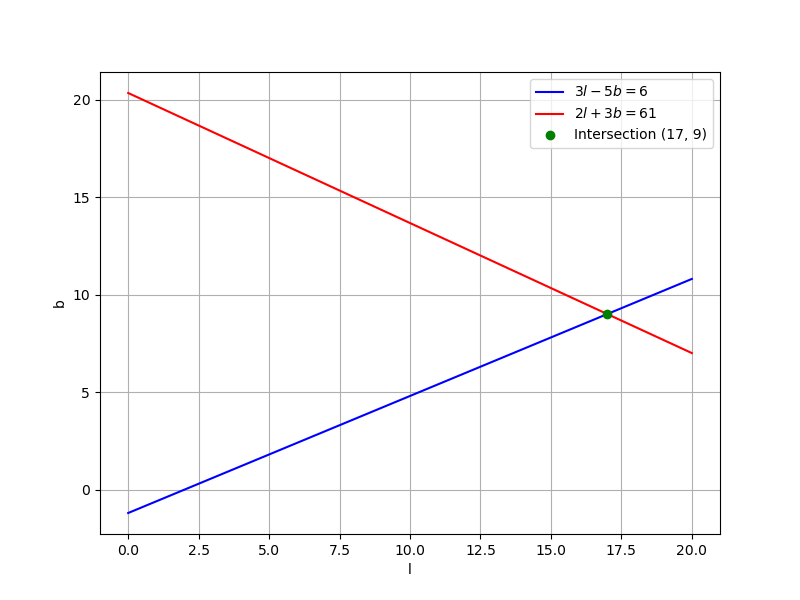
\includegraphics[width=\columnwidth]{fig/plot.png}
    \label{figure:1.1}
\end{figure}


\end{document}
